\section{Method}
We use the Faster R-CNN model with ResNet50 as the backbone for our model. Moreover, the Feature Pyramid Network (FPN) module is used to improve our solution. The Faster R-CNN is a real-time object detection model, which consists of $2$ modules. The first module of the Faster R-CNN model is a deep fully convolutional network that proposes regions. The second module is a detector that uses proposed regions from the first one \cite{f-rcnn}. This is a single, unified network for object detection. By using the recently popular terminology of neural networks as the 'attention' mechanisms, the Region Proposal Networks (RPN) tells the Faster R-CNN where to look.

\begin{figure}[H]
\centering{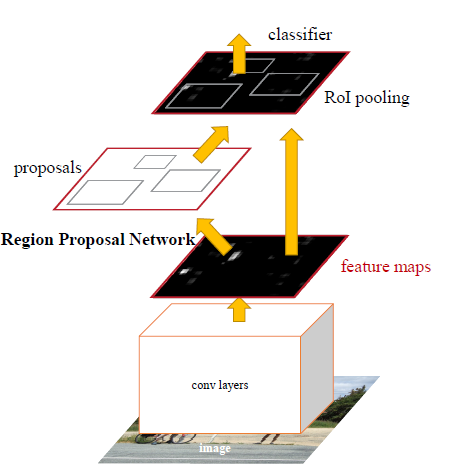
\includegraphics[scale=0.7]{faster-rcnn/faster-rcnn}}
\caption{Faster R-CNN is a single, unified network for object detection. The RPN module plays the role of the 'attention' of this network. \cite{f-rcnn}}
\end{figure}
\newpage
\subsection{Region Proposal Networks}
An RPN takes an image as input and outputs a set of rectangular object proposals each with an objectness score, which measures membership to a set of object classes. This process is modeled with a fully convolutional network. The structure of the RPN is shown in Figure \ref{rpn}, and figure \ref{rpn_example} shows some examples of object detection using RPN proposals, on the PASCAL VOC 2007 test. The method introduced in  \cite{f-rcnn} detects objects in a wide range of scales and aspect ratios.

\begin{figure}[H]
\centering{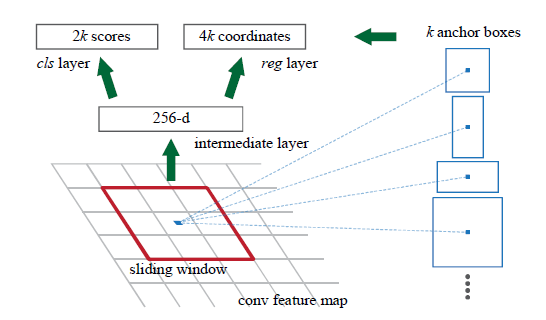
\includegraphics[scale=.8]{faster-rcnn/rpn}}
\caption{Region Proposal Network (RPN) \cite{f-rcnn}}
\label{rpn}
\end{figure}

\begin{figure}[H]
\centering{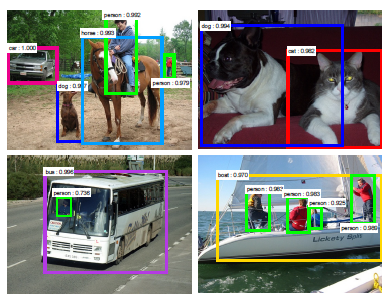
\includegraphics[scale=.8]{faster-rcnn/rpn_example}}
\caption{Examples of object detection using RPN proposals \cite{f-rcnn}}
\label{rpn_example}
\end{figure}

\textbf{Loss function:} From \cite{f-rcnn}, the loss function of the RPN is:
$$\begin{gathered}
L\left( {\left\{ {{p_i}} \right\},\left\{ {{t_i}} \right\}} \right) = \frac{1}{{{N_{cls}}}}\sum\limits_i {{L_{cls}}\left( {{p_i},p_i^*} \right)}  \hfill \\
 + \lambda \frac{1}{{{N_{reg}}}}\sum\limits_i {p_i^*} {L_{reg}}\left( {{t_i},t_i^*} \right). \hfill \\
\end{gathered} $$

\subsection{Sharing Features for RPN and Fast R-CNN}
In the Faster R-CNN model, they use a 4-step training algorithm to learn shared features via alternating optimization \cite{f-rcnn}. In the first step, the RPN is trained end-to-end by back-propagation and stochastic gradient descent (SGD). In the second step, they train a separate detection network by Fast R-CNN. In the third step, they use the detector network to initialize RPN training, and they let the two networks share convolutional layers. Finally, they keep the shared convolutional layers fixed, they fine-tune the unique layers of Fast R-CNN.

\subsection{ResNet50}
ResNet50 is a variant of the ResNet model, consisting of $48$ convolution layers with $1$ MaxPool and $1$ Average Pool layer. It has $3.8 \times 10^9$ floating points operations. The ResNet50 is a widespread ResNet model. \\
\begin{table*}
\caption{\label{resnet50} ResNet50 architecture \cite{resnet-50}}
\begin{tabularx}{\textwidth}{|c|c|c|c|c|c|c|}
\hline
layer name & output size      & \multicolumn{1}{c|}{18-layer}                                                                                                                                                                                                                                                                                                          & \multicolumn{1}{c|}{34-layer}                                                                                                                                                                                                                                                                                                          & \multicolumn{1}{c|}{50-layer}                                                                                                                                                                                                                                                                                                                                                                                & \multicolumn{1}{c|}{101-layer}                                                                                                                                                                                                                                                                                                                                                                               & 152-layer                                                                                                                                                                                                                                                                                                                                                                               \\ \hline
conv1      & $112 \times 112$ & \multicolumn{5}{c|}{$7 \times 7,$ 64, stride 2}                                                                                                                                                                                                                                                                                                                                                                                                                                                                                                                                                                                                                                                                                                                                                                                                                                                                                                                                                                                                                                                                                                                                                                                                                                                                                                                                                                                                                                                                                                                                                                                                                                                                                                                                                                                                                                                         \\ \hline
conv2$\_$x & $56 \times 56$   & 
$\left[ {\begin{array}{*{20}{c}}

  {3 \times 3,64} \\ 

  {3 \times 3,64} 

\end{array}} \right] \times 2$ & 
$\left[ {\begin{array}{*{20}{c}}

  {3 \times 3,64} \\ 

  {3 \times 3,64} 

\end{array}} \right] \times 3$ & 
$\left[ {\begin{array}{*{20}{c}}
  {1 \times 1,64} \\ 
  {3 \times 3,64} \\ 
  {1 \times 1,256} 
\end{array}} \right] \times 3$ & 
$\left[ {\begin{array}{*{20}{c}}
  {1 \times 1,64} \\ 
  {3 \times 3,64} \\ 
  {1 \times 1,256} 
\end{array}} \right] \times 3$  & 
$\left[ {\begin{array}{*{20}{c}}
  {1 \times 1,64} \\ 
  {3 \times 3,64} \\ 
  {1 \times 1,256} 
\end{array}} \right] \times 3$ 
\\ \hline
conv3$\_$x  & $28 \times 28$ & 
$\left[ {\begin{array}{*{20}{c}}

  {3 \times 3,128} \\ 

  {3 \times 3,128} 

\end{array}} \right] \times 2$ & 
$\left[ {\begin{array}{*{20}{c}}

  {3 \times 3,128} \\ 

  {3 \times 3,128} 

\end{array}} \right] \times 4$ & 
$\left[ {\begin{array}{*{20}{c}}
  {1 \times 1,128} \\ 
  {3 \times 3,128} \\ 
  {1 \times 1,512} 
\end{array}} \right] \times 4$ &
$\left[ {\begin{array}{*{20}{c}}
  {1 \times 1,128} \\ 
  {3 \times 3,128} \\ 
  {1 \times 1,512} 
\end{array}} \right] \times 4$  &
$\left[ {\begin{array}{*{20}{c}}
  {1 \times 1,128} \\ 
  {3 \times 3,128} \\ 
  {1 \times 1,512} 
\end{array}} \right] \times 8$                                                                                                                                                                                                                                                                                                                                                                                         \\ \hline
conv4$\_$x & $14 \times 14$ &
$\left[ {\begin{array}{*{20}{c}}

  {3 \times 3,256} \\ 

  {3 \times 3,256} 

\end{array}} \right] \times 2$  &
$\left[ {\begin{array}{*{20}{c}}

  {3 \times 3,256} \\ 

  {3 \times 3,256} 

\end{array}} \right] \times 6$  & 
$\left[ {\begin{array}{*{20}{c}}
  {1 \times 1,256} \\ 
  {3 \times 3,256} \\ 
  {1 \times 1,1024} 
\end{array}} \right] \times 6$ & 
$\left[ {\begin{array}{*{20}{c}}
  {1 \times 1,256} \\ 
  {3 \times 3,256} \\ 
  {1 \times 1,1024} 
\end{array}} \right] \times 23$ &                                                                                                                                                                                                                                                                                                                                                                                
$\left[ {\begin{array}{*{20}{c}}
  {1 \times 1,256} \\ 
  {3 \times 3,256} \\ 
  {1 \times 1,1024} 
\end{array}} \right] \times 36$         
\\ \hline
conv5$\_$x & $7 \times 7$ & 
$\left[ {\begin{array}{*{20}{c}}

  {3 \times 3,512} \\ 

  {3 \times 3,512} 

\end{array}} \right] \times 2$ &
$\left[ {\begin{array}{*{20}{c}}

  {3 \times 3,512} \\ 

  {3 \times 3,512} 

\end{array}} \right] \times 6$  &
$\left[ {\begin{array}{*{20}{c}}
  {1 \times 1,512} \\ 
  {3 \times 3,512} \\ 
  {1 \times 1,2048} 
\end{array}} \right] \times 3$  &
$\left[ {\begin{array}{*{20}{c}}
  {1 \times 1,512} \\ 
  {3 \times 3,512} \\ 
  {1 \times 1,2048} 
\end{array}} \right] \times 3$  &                                                                                                                                                                                                                                                                                                                                                                                        
$\left[ {\begin{array}{*{20}{c}}
  {1 \times 1,512} \\ 
  {3 \times 3,512} \\ 
  {1 \times 1,2048} 
\end{array}} \right] \times 3$ 
\\
\hline
\multicolumn{1}{|c|}{} & $1 \times 1$ & \multicolumn{5}{c|}{average pool, 1000-d fc, softmax}                                                                                                                                            \\ \hline
\multicolumn{2}{|c|}{FLOPs}           & \multicolumn{1}{c|}{$1.8 \times {10^9}$} & \multicolumn{1}{c|}{$3.6 \times {10^9}$} & \multicolumn{1}{c|}{$3.8 \times {10^9}$} & \multicolumn{1}{c|}{$7.6 \times {10^9}$} & $11.3 \times {10^9}$ \\ \hline
\end{tabularx}
\end{table*}
Table \ref{resnet50} shows the architecture of the ResNet50.
We can see that \cite{resnet-50}, in a ResNet50 architecture, there are:
\begin{itemize}
\item A convolution with a kernel size of $7 \times 7$ and $64$ different kernels all with a stride of size $2$ there is $1$ layer.
\item Next there is a max pool with also a stride size of 2.
\item In the next convolution there is a $1 \times 1$, $64$ kernel following this a $3 \times 3$, $64$ kernel and at last a $1 \times 1$, $256$ kernel. These three layers are repeated in total $3$ times so there are $9$ layers in this step.
\item Next we see a kernel of $1 \times 1$, $128$ after that a kernel of $3 \times 3$, $128$ and at last a kernel of $1 \times 1$, $512$ this step was repeated $4$ times so there are $12$ layers in this step.
\item After that there is a kernel of $1 \times 1$, $256$ and two more kernels with $3 \times 3$, $256$ and $1 \times 1$, $1024$ and this is repeated $6$ times there are a total of $18$ layers.
\item And then again a $1 \times 1$, $512$ kernel with two more of $3 \times 3$, $512$ and $1 \times 1$, $2048$ and this was repeated $3$ times there are a total of $9$ layers.
\item After that we do an average pool and end it with a fully connected layer containing $1000$ nodes and at the end a softmax function so this gives us $1$ layer.
\end{itemize}
There are $1 + 9 + 12 + 18 + 9 + 1 = 50$ layers in total.
\subsection{Feature Pyramid Network}
The Feature Pyramid Network (FPN) is used to address the problem of the large-scale span. The task of Mathematical Formulas Detection (MFD) contains a large number of extremely small formulas, which brings great challenges for us. As shown in figure \ref{fpn} \cite{1stprize}, for a single extremely small character formula, its short side is usually about $16$ pixels. We discover that for any layer of FPN, the limit of the detector is $3$ pixels, which means that if we use the default ($3$-$7$), the short side needs to be at least $24$ pixels to be detected. It can be seen clearly that there are many small embedded formulas that do not satisfy this condition. As a result, we have changed the selection of the FPN level to ($2$-$6$), so that our model can overcome this challenge.
\begin{figure}[H]
\centering{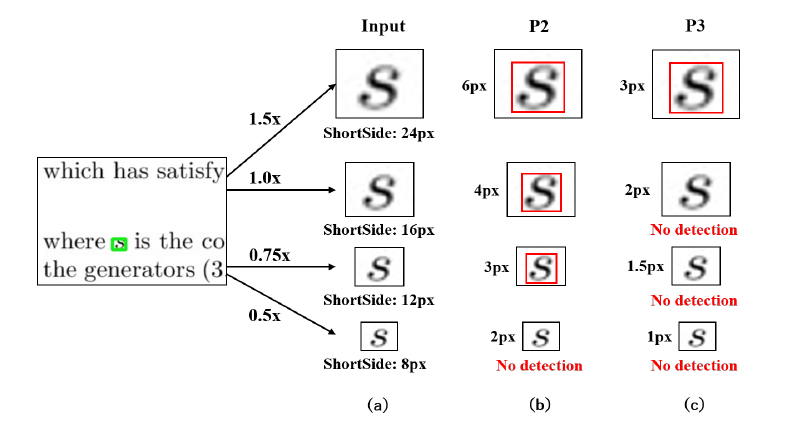
\includegraphics[scale=.5]{faster-rcnn/fpn}}
\caption{The significance of FPN in the task of MFD. (a) Input size; (b): Corresponding size in P2, (c) Corresponding size in P3. Under some small cases, some positive samples will be missed \cite{1stprize}}
\label{fpn}
\end{figure}
